%!TEX root = ../main.tex
\section{Inputs/Sensoren}
 \frame{\sectionpage}

\begin{frame}{Kameras}

Wir verwenden hauptsaechlich webcams da die einbindung in einen realtime kontext am einfachsten/gängigsten ist.

\end{frame}


\begin{frame}{Mikrophone}
\begin{itemize}
	\item 'Übliche' Mikrophone
	\item piezo mikrophone (Körperschall)
	\item mehrkanal setups (zb. mic arrays)
\end{itemize}
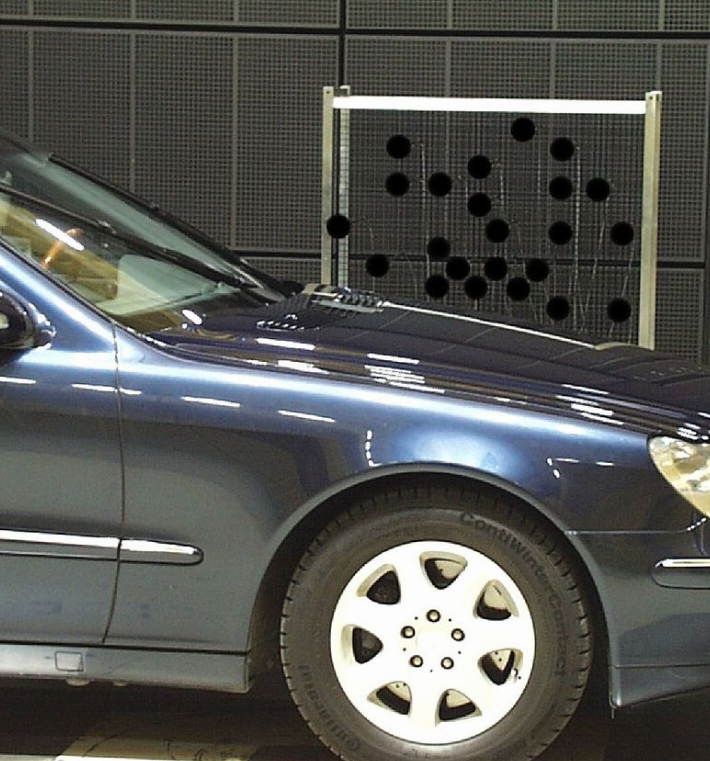
\includegraphics[width=\textwidth]{micarr.png}

\end{frame}


\begin{frame}{3D Cameras}
\begin{itemize}
	\item intel real sense
	\item kinect
	\item nicht vergessen: K.I. benutzen um 3D info zu schätzen. z.B. 'Posenet'.
\end{itemize}
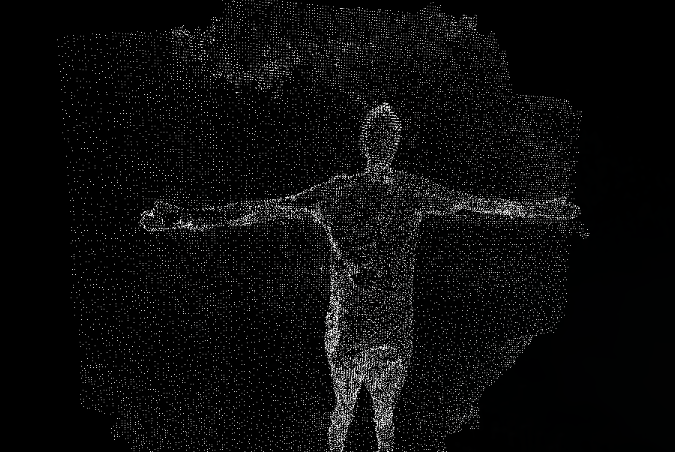
\includegraphics[width=\textwidth]{pcloud.png}
\end{frame}

\begin{frame}{HID (Human Interface devices)}
	\begin{itemize}
		\item Computer keyboard 
		\item Diverse Midi controller
		\item Touchscreens
		\item div. potentiometer (nicht zwangsläufig MIDI)
		\item Eye-tracking
		\item handtracking (-> 'leap motion')
		\item 3d tracking im raum (zb. Vive controller)
		\item ...
	\end{itemize}
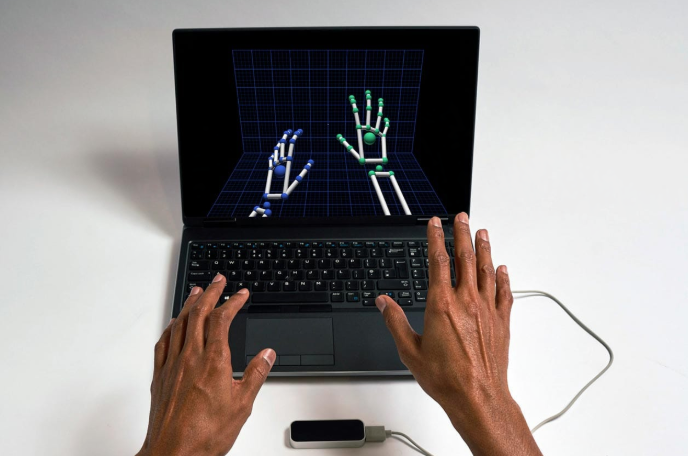
\includegraphics[width=5cm]{leap.png}
\end{frame}


\begin{frame}{Sonstige Sensoren}

\begin{columns}
	\begin{column}{0.5\textwidth}
		\begin{itemize}
		\item Accelerometer
		\item Thermometer
		\item Ultraschall distanzmesser
		\item Photoresistoren
		\item ....
		\end{itemize}
	\end{column}

	\begin{column}{0.5\textwidth}
		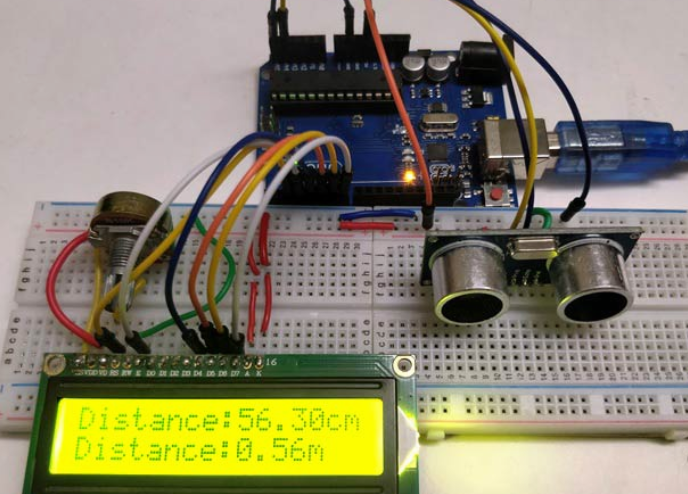
\includegraphics[width=5cm]{dist.png}
	\end{column}

\end{columns}

\end{frame}

\begin{frame}{APIs und open data}
\end{frame}

\section{Outputs/Dispositive}
 \frame{\sectionpage}

\begin{frame}{Screens}

\end{frame}


\begin{frame}{Projektoren}
\begin{itemize}
	\item Standard Projektion
	\item 3D Projektion (shutter brillen etc)
	\item 2d/3D Mapping
	\item Räumliche Dispositive (z.B. Fulldome)
	\item 'Hologramme'
\end{itemize}
\begin{center}

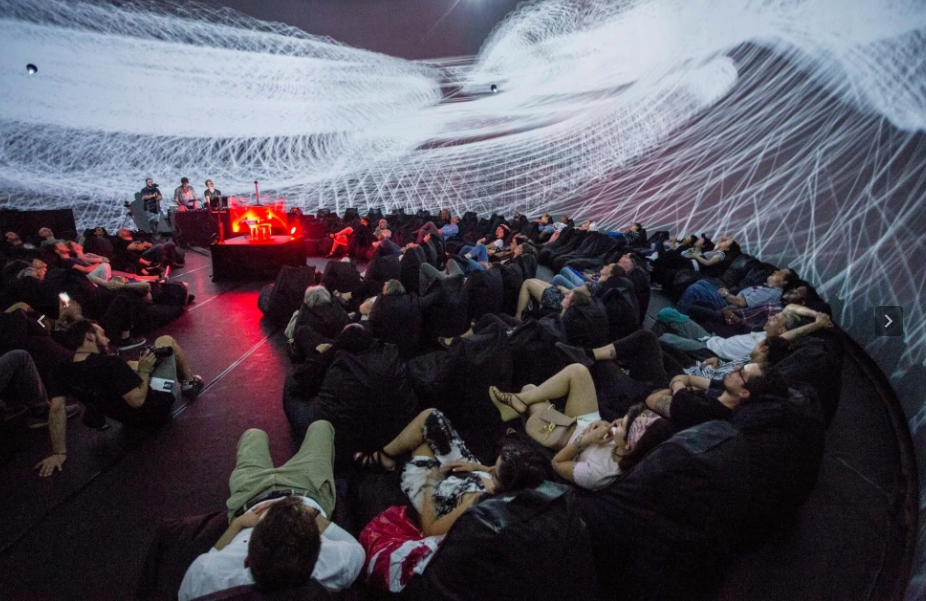
\includegraphics[width=7cm]{dome.png}
\end{center}
\end{frame}


\begin{frame}{Lautsprecher, Kopfhoerer}

\end{frame}

\begin{frame}{Sonstiges}
\begin{itemize}
	\item Professionelle Lichtanlagen (DMX)
	\item Licht, LED strips
	\item Motoren, pumpen etc

\end{itemize}

\end{frame}



